\documentclass[10pt,a4paper]{article}
\usepackage[utf8]{inputenc}
\usepackage[a4paper]{geometry}
\usepackage{fullpage}
\usepackage{multicol}
\usepackage[usenames,dvipsnames]{color}
\usepackage{graphicx}
%\usepackage[landscape]{geometry}
%needs to be defined before using the pdftex package
\definecolor{linkcolor}{rgb}{0.1,0.0,0.35}
\definecolor{citecolor}{rgb}{0.1,0.0,0.35}
\definecolor{unchangedcolor}{rgb}{0.4,0.4,0.4}
%\definecolor{unchangedcolor}{rgb}{0.2,0.2,0.6}
\definecolor{changedcolor}{rgb}{1.0,0.2,0.0}
\usepackage[pdftex,
            colorlinks=true,
            linkcolor=linkcolor,
            filecolor=red,
            citecolor=citecolor,
            pdftitle={TLAPM v2 Architecture},
            pdfauthor={Martin Riener},
            pdfsubject={},
            pdfkeywords={},
            bookmarks, bookmarksnumbered=true]{hyperref}
\usepackage{cite}
\usepackage{url}

\title{TLAPM v2 Architecture}

\begin{document}
\maketitle

\section{Introduction}
\label{sec:introduction}
The TLA Proof Manager (PM) reads a TLA+ specification and extracts the
 expressions needed to prove the steps of its theorems. These expressions are
 called proof obligations. A backend convert an obligation into suitable
 input for a theorem prover. At the moment, there exist backends for
 Isabelle/TLA, Zenon, SMT and LS4 where each of them covers a different subset
 of the language.

The rewrite of the PM adresses the following problems:

\begin{itemize}
\item Properties about ENABLED can only be proved by coalescing (which is
 incomplete)
\item Temporal quantifiers don't have backend
\item Recursively defined operators are not expanded
\item The data-structures of the current PM are mutable and have deBruijn
 indices, making debugging exceptionally complicated
\item The languages accepted by toolbox and the PM need to agree. In case of
 conflicting interpretations, the language accepted by the toolbox is
 authoritative. The easiest way to prevent disagreement is to share the parser
 between the toolbox and the PM.
\end{itemize}


\section{General Architecture}
\label{sec:general}

SANY, the abstract syntax tree used in the toolbox, is implemented in Java,
 wheras the PM is implemented in OCaml. The first step is to serialze the Java
 datastructures to XML and recreate them in OCaml (see section \ref{sec:sany}).
 Since the SANY datastructures are considered as static, the second step
 converts them to the internal syntax tree (see section \ref{sec:exprds}).
 After applying some processing steps, the specification is divided into
 a list of obligations. The backends (section \ref{sec:backends}) are resposible
 for exporting an obligation to a theorem prover and the quering of the results.
 The status of each obligation proof attempt is communicated back to the Toolbox
 via standard output using a text-based protocol (section \ref{sec:protocol}).

 \begin{figure}[htb]
   \centering
   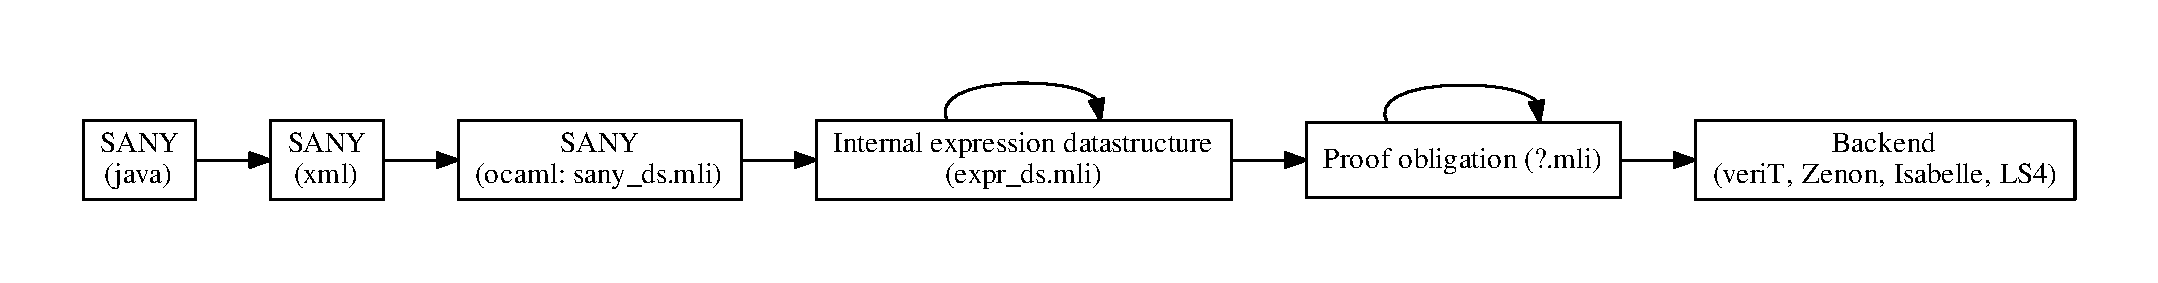
\includegraphics[width=\textwidth]{architecture.pdf}
   \caption{Architecture Overview - Data Structures}
   \label{fig:datastructures}
 \end{figure}
\section{SANY Import (sany\_*.mli)}
\label{sec:sany}

\section{Internal Datastructure (expr\_*.mli)}
All of these are universal for the whole spec:
\label{sec:exprds}
\begin{itemize}
\item Resolve explicit substitutions
 (Problem: does not distribute over ENABLED?)
\item $\beta$-reduce lambda expressions
\item $\lambda$-abstraction is realized as application. replace by explicit
 lambda operator (an expression).
\item replace @ notation by the expressions they stand for
\item replace ! notation by what it refers to
\item  let-in?
\item remove theorems from submodules, replace named theorems by user-defined
 operators
\end{itemize}

\section{Obligations}
\label{sec:obligations}

The unfolding of definitions is the single transformation which depends on the
 proof context. Together with the list of declared operators, the ASSUME-PROVE
 statement of a theorem with onfolded definitions forms a proof obligation.

Since what is coalesced depends on the capabilities of the backend, it also
 applies to an obligation.
\section{Backends}
\label{sec:backends}

\section{Toolbox Protocol}
\label{sec:protocol}


\end{document}
